\documentclass[12pt]{article}
%Gummi|065|=)
\usepackage{amsmath, amsfonts, amssymb}
\usepackage[margin=0.5in]{geometry}
\usepackage{xcolor}
%\usepackage{graphicx}
%\usepackage{graphicx}
\newcommand{\off}[1]{}
\DeclareMathSizes{20}{30}{21}{18}

\newcommand{\myhrule}{}

\newcommand{\dash}{
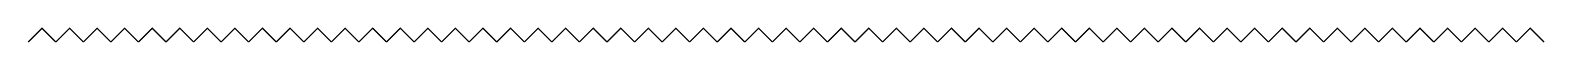
\begin{tikzpicture}[scale=0.35]
\foreach \x in {1,...,55}{
	\draw (\x,-0.25)--(\x+0.5,0.25)--(\x+1,-0.25);
}
\end{tikzpicture}
}

\usepackage{tikz}

\title{\textbf{ Examples: The Matrix-Tree Theorem}}
\author{John D Mangual}
\date{}
\begin{document}

\fontfamily{qag}\selectfont \fontsize{25}{30}\selectfont

\maketitle

\fontfamily{qag}\selectfont \fontsize{12}{10}\selectfont

\noindent On YouTube there are some nice videos of Francis Brown lecturing on the ``Cosmic Galois Group".  I know a little bit about a few of these things:
\begin{itemize}
\item periods (integrals of stuff)
\item the matrix-tree theorem
\item Feynman Diagrams
\item $\zeta(2) = \sum \frac{1}{n^2} = \frac{\pi^2}{6}$ 
\begin{itemize}
\item the Feynman diagram evaluates to some zeta functions
\item the zeta function can be represented as a period
\end{itemize}
\item Things I like such as $\zeta(-1) = 1 + 2 + 3 + \dots = - \frac{1}{12}$
\end{itemize}
Before we get too exicted let's discuss the questions at hand. \\ \\
\textbf{Problem \#1} -- What?? Don't we know how to compute Feynman diagrams already? \\ \\
\textbf{Problem \#2} -- Which QFT is Brown\footnote{ or Panzer or Schnetz or Block or Broadhurst or Kreimer} referring to? \\ \\
Brown refers to the Matrix Theorem while defining is Feynman Amplitudes -- but \textit{which Feynman amplitudes} -- it is not obvious to me this is plain-old $\phi^4$ theory. \\ \\
\begin{itemize}
\item $\mathbf{\phi}^4$ theory is what my Physics teacher glossed over, a trivial and generate case and an endless source of homework problems.  So obviously we know all about that. \\ \\
\item After some research there is the thesis of Eric Panzer who refers to the \textbf{Schwinger Trick} -- basically a Mellin transform -- turning Feynman diagrams into sums over spanning trees.  \textbf{\color{green!80!black!80!white} which Schwinger trick}?\;\footnote{Due to my limited knowledge of QFT.  Depending on who teaches the course, you get a different version of the story.}
\end{itemize}
So\dots comparing Brown's approach to Chapter 4 of Peskin and Schroeder leads to a lot of confusion which we hopefully can resolve.  \\ \\Also, Brown is looking to evaluate all diagrams I will only look at few such as 
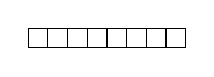
\begin{tikzpicture}[scale=0.25]
\draw (0,0)--(8,0)--(8,1)--(0,1)--cycle;
\foreach \a in {1,2,3,4,5,6,7}{
\draw (\a,0)--(\a,1);
}
\end{tikzpicture}
and
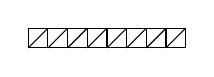
\begin{tikzpicture}[scale=0.25]
\draw (0,0)--(8,0)--(8,1)--(0,1)--cycle;
\foreach \a in {0,1,2,3,4,5,6,7}{
\draw (\a,0)--(\a+1,1);
}
\foreach \a in {1,2,3,4,5,6,7}{
\draw (\a,0)--(\a,1);
}
\end{tikzpicture}

\newpage


\noindent As along as I can find some textbook which contain this idea which he attributes to Schwinger, I am able to continue writing.
\begin{itemize}
\item the schwinger trick must be pretty good if its the basis for a theory.  Spencer Bloch, Helene and Dirk Kreimer  point to Zuber's textbook (in the bibliography)
\item Feynman Diagrams are a part of \textbf{perturbation theory} and I have found a nice discussion in Chapter 6-2 on \textbf{diagrammatics}
\end{itemize}
This is not a deep philosophical book.  I need to know which book to look at and which equations to copy. \\ \\ \dash
\\ \\
- equations -

\newpage

\fontfamily{qag}\selectfont \fontsize{12}{10}\selectfont

\begin{thebibliography}{}

\item Francis Brown \textbf{Feynman Amplitudes and Cosmic Galois group} \texttt{arXiv:1512.06409}

\item Francis Brown \textbf{Notes on Motivic Periods}
\texttt{arXiv:1512.06410}

\item Michael Peskin, Daniel Schroeder \textbf{Quantum Field Theory} (Student Economy Edition), 2015

\item Spencer Bloch, H\'{e}l\`{e}ne Esnault, Dirk Kreimer.\textbf{On Motives Associated to Graph Polynomials.}
\texttt{math/0510011}

\item Claude Itzykson, Jean-Bernard Zuber \textbf{Quantum Field Theory} McGraw-Hill, 1980.

\end{thebibliography}



\end{document}